%% Results, part 2: privileged distillation, hard mining, unseen families, ablations and cost.
%% Included by sigconf.tex. Do not add a preamble here.

\subsection{Privileged observation self-distillation provides complementary information}
\label{sec:q-posd}

\textbf{Claim.} A richer training-time observation of the same history improves the deployment-constrained student
where exposure to process variation does not, namely when the task is information limited and the student underfits
rather than overfits to one observation pattern.

\textbf{Evidence.} Table~\ref{tab:posd} isolates the mechanism on USHCN at a one-month horizon, the setting where
augmentation is least effective. Adding privileged distillation on top of augmentation lowers clean MSE from
$0.53287$ to $0.51348$ ($-3.6\%$) and mean shifted MSE from $0.54379$ to $0.52662$ ($-3.2\%$), and it improves
every one of the fifteen shifted conditions. It is the only mechanism we measure that improves the clean condition
by more than noise. On the twelve-month horizon the complete configuration, which includes distillation, likewise
improves clean MSE from $0.52020$ to $0.51686$. On P19 the complete configuration raises clean AUROC from $82.13$
to $85.59$ and AUPRC from $16.89$ to $24.47$, the largest accuracy gain in the paper; because only the complete
configuration was run on P19 we cannot attribute that gain to distillation alone, though P19's severe class
imbalance is the same information-limited regime. On PhysioNet, by contrast, distillation is within noise of
augmentation on shifted error and slightly worse on clean error
($0.00573$ vs.\ $0.00553$, Table~\ref{tab:components}).

\textbf{Interpretation.} The effect is an accuracy effect, not a robustness effect: on USHCN the relative
degradation $\Delta_{\mathrm{shift}}$ does not improve when distillation is added ($+2.0\%\rightarrow+2.6\%$) even
as absolute error falls at every condition. This is what we would expect if the teacher's output acts as a target
that is easier to fit than the raw future, supplying information about the trajectory that the student's own view
leaves ambiguous. Where the sparse observation already determines the target well, as on PhysioNet, there is
little for the richer observation to add, and the extra term is inert. The two mechanisms are therefore
complementary rather than substitutable, and neither subsumes the other.

\begin{table}[t]
\caption{Privileged observation self-distillation on USHCN at a one-month horizon (test MSE\prelim), the setting
where augmentation alone is least effective. The distillation row differs from the augmentation row only in the
added term of Eq.~\ref{eq:distill}.}
\label{tab:posd}
\small
\begin{tabular}{lrrrr}
\toprule
configuration & clean & mean shift & worst & $\Delta_{\mathrm{shift}}$ \\
\midrule
no mechanism & 0.53787 & 0.54808 & 0.56933 & $+1.9\%$ \\
augmentation & 0.53287 & 0.54379 & 0.56959 & $+2.0\%$ \\
\quad $+$ distillation & \textbf{0.51348} & \textbf{0.52662} & 0.54877 & $+2.6\%$ \\
\quad $+$ mining & 0.52656 & 0.54754 & 0.56888 & $+4.0\%$ \\
all three & 0.52107 & 0.52871 & \textbf{0.54584} & $\mathbf{+1.5\%}$ \\
\bottomrule
\end{tabular}
\end{table}

\subsection{Hard-process mining helps only when its pool exceeds the training pool}
\label{sec:mining-results}

\textbf{Claim.} Searching for worst-case observation processes improves worst-case error, but only when the
candidate pool contains processes meaningfully harsher than those augmentation already draws.

\textbf{Evidence.} With $\mathcal{P}=P_{\mathrm{mix}}$, the natural default, mining is indistinguishable from
augmentation on PhysioNet: $\Delta_{\mathrm{shift}}$ of $+14.8\%$ against $+14.3\%$, mean shifted MSE of
$0.00641$ against $0.00632$, at $2.7\times$ the training time (Tables~\ref{tab:components} and \ref{tab:cost}).
With a pool containing severities and pairwise compositions absent from $P_{\mathrm{mix}}$, the same mechanism
becomes the strongest single configuration we obtain on PhysioNet on both mean shifted error and worst-case error
($0.00626$ and $0.00721$), and the gain concentrates where the mechanism targets: $0.00706$ against $0.00747$
under 70\% dropout, and $0.00721$ against $0.00753$ under 50\% variable removal.

\textbf{Interpretation.} The hardest of $K$ draws from the training mixture is barely harder than one draw, so
with a matched pool the maximisation in Eq.~\ref{eq:mining} has nothing to find and the mechanism reduces to
augmentation at $K$ times the cost. Severity of the pool, not the search, is what produces the improvement. This
is why we name two configurations rather than one. OPERA is augmentation plus privileged distillation, with no
pool to choose. OPERA++ adds mining from a strictly harsher pool, and is the configuration to use when worst-case
error is what matters. Mining from the matched pool is neither, and we report it only as the control that
establishes the distinction; a reader who adopted it as the default would pay $K$ forward passes per step for
nothing. The boundary on OPERA++ should be stated plainly as well: its advantage over OPERA is $0.00006$\,MSE at
one seed, it introduces a second pool that must stay disjoint from evaluation, and on USHCN mining without
distillation is the worst configuration in Table~\ref{tab:posd}.

\subsection{Robustness extends to unseen observation-process families}
\label{sec:q-unseen}

\textbf{Claim.} The gain is generalisation across observation processes rather than memorisation of the training
pool.

\textbf{Evidence.} Table~\ref{tab:unseen} and Figure~\ref{fig:unseen} split the shifted conditions into those
whose family appears in the training pool, at severities outside it, and the nine whose family never appears at
all. Without any mechanism the two groups are both far above clean error and the unseen group is worse
($0.01260$ against $0.00975$). With augmentation the three columns are nearly level ($0.00553$, $0.00603$,
$0.00652$), and the residual unseen-minus-seen gap is $0.0005$\,MSE against $0.0029$\,MSE for the baseline. The
single clearest case is temporal subsampling, which appears in the training pool only at stride $2$: baseline
error at stride $3$ is $0.00923$ and with augmentation $0.00572$, against a clean error of $0.00553$.

\textbf{Interpretation.} Exposure to a mixture of removal structures generalises to removal structures outside
the mixture, which suggests the student is learning to use whatever observations remain rather than learning the
specific patterns it was trained on. The caveat is that our unseen families are drawn from the same nine-primitive
vocabulary as the training pool, so this is evidence of generalisation across families within one family space and
not of generalisation to an arbitrary new acquisition regime.

\begin{table}[t]
\caption{Generalisation across the observation-process split on PhysioNet (test MSE\prelim). ``seen'' averages the
four conditions whose family and severity range the training pool covers; ``unseen'' averages the nine conditions
whose family never appears in training.}
\label{tab:unseen}
\small
\begin{tabular}{lrrrr}
\toprule
configuration & clean & seen & unseen & unseen $-$ seen \\
\midrule
no mechanism & \textbf{0.00549} & 0.00975 & 0.01260 & $0.00285$ \\
augmentation & 0.00553 & \textbf{0.00603} & 0.00652 & $0.00049$ \\
\quad $+$ distillation & 0.00573 & 0.00619 & 0.00662 & $0.00043$ \\
\quad $+$ mining, harsher pool & 0.00562 & 0.00607 & \textbf{0.00640} & $\mathbf{0.00033}$ \\
all three & 0.00559 & 0.00606 & 0.00650 & $0.00044$ \\
\bottomrule
\end{tabular}
\end{table}

\begin{figure}[t]
\centering
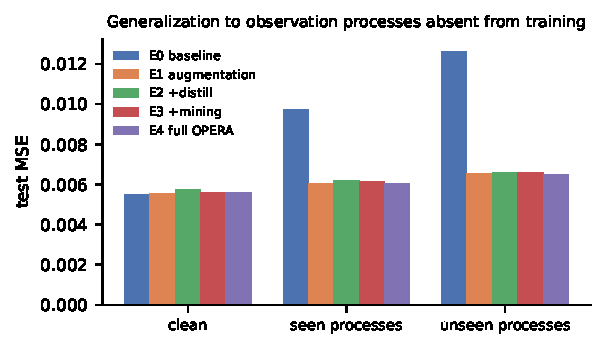
\includegraphics[width=0.85\linewidth]{figures/fig4_unseen_generalization.pdf}
\caption{The split of Table~\ref{tab:unseen} on PhysioNet\prelim. The gap between the seen and unseen bars is
small for every configuration trained with observation-process augmentation and large without any mechanism.}
\label{fig:unseen}
\end{figure}

\subsection{Ablations and cost}
\label{sec:q-cost}

\paragraph{Robustness is not bought with in-distribution accuracy.}
Figure~\ref{fig:ablation} places mean degradation under shift against clean error for every PhysioNet
configuration. Degradation falls by roughly an order of magnitude while clean error moves within
$0.0004$\,MSE, so no configuration is trading accuracy on the dataset's own observation process for robustness to
others. The one exception is the combination of all three mechanisms with the harsher mining pool, whose clean
error is $0.00590$ against the baseline's $0.00549$; that configuration attains the lowest
$\Delta_{\mathrm{shift}}$ in Table~\ref{tab:components} and the highest clean error among our configurations,
which is the clearest illustration in our results of why the ratio must not be read alone.

\paragraph{Representation matching is not used.}
Our implementation also supports distilling representations instead of predictions. We report it only as an
ablation and do not include it in any configuration above, because it reimposes exactly the cross-view latent
equality that Section~\ref{sec:aug} declines to require.

\paragraph{Cost.}
Table~\ref{tab:cost} reports overhead. Every mechanism is training-time only: parameter count is identical across
configurations and inference latency is unchanged at $0.63$\,ms per series, so the deployed model is the
unmodified encoder. Augmentation costs $1.7\times$ training time and $1.7\times$ peak memory for $V=2$ views;
distillation adds one forward pass and no gradient memory; mining adds $K$ scoring passes.

\begin{figure}[t]
\centering
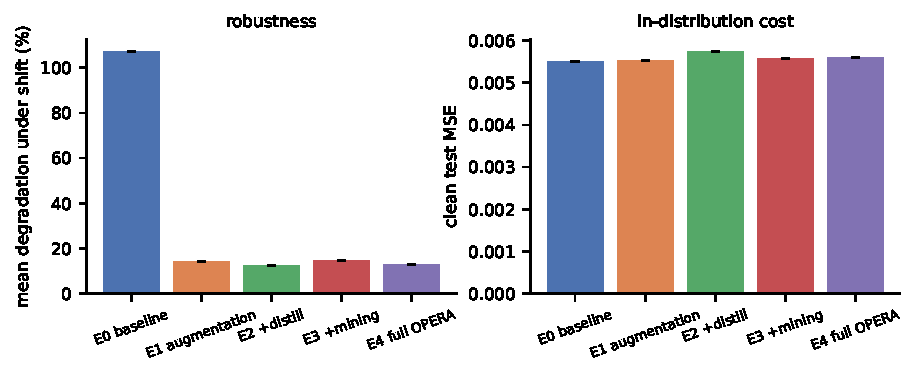
\includegraphics[width=\linewidth]{figures/fig5_ablation.pdf}
\caption{Contribution of each mechanism on PhysioNet\prelim: mean degradation under shift (left, lower is better)
against in-distribution error (right).}
\label{fig:ablation}
\end{figure}

\begin{table}[t]
\caption{Training and deployment cost on PhysioNet\prelim. Inference latency and parameter count are unaffected by
every mechanism.}
\label{tab:cost}
\small
\begin{tabular}{lrrrr}
\toprule
configuration & params & s/epoch & peak GB & infer.\ ms \\
\midrule
no mechanism & 129{,}153 & 24.1 & 3.7 & 0.630 \\
augmentation & 129{,}153 & 41.4 & 6.3 & 0.670 \\
$+$ distillation & 129{,}153 & 45.3 & 6.3 & 0.630 \\
$+$ mining (harsher pool) & 129{,}153 & 82.3 & 6.3 & 0.634 \\
all three (harsher pool) & 129{,}153 & 86.3 & 6.3 & 0.629 \\
\bottomrule
\end{tabular}
\end{table}
